\section*{CHAPTER 2. THEORETICAL BACKGROUND}
\addcontentsline{toc}{section}{\numberline{}CHAPTER 2. THEORETICAL BACKGROUND}

\setcounter{section}{2}
\setcounter{subsection}{0}
\setcounter{figure}{0}
\setcounter{table}{0}
\setcounter{equation}{0}

%============================================================%
\subsection{Overview of Multicarrier Transmission}

Modern wireless communication systems operate in environments affected by
multipath propagation, delay spread, Doppler effects, and additive noise.
These impairments introduce inter-symbol interference (ISI) and degrade
transmission reliability, especially at high data rates.

Conventional single-carrier systems require complex time-domain
equalization to compensate for frequency-selective fading channels.
As bandwidth increases, equalizer complexity grows significantly.

To overcome this limitation, multicarrier transmission techniques divide
the available bandwidth into multiple narrowband orthogonal subcarriers.
Instead of transmitting one high-rate stream, the input data stream is
split into several parallel low-rate streams.

\vspace{0.3cm}

\begin{figure}[H]
    \centering
    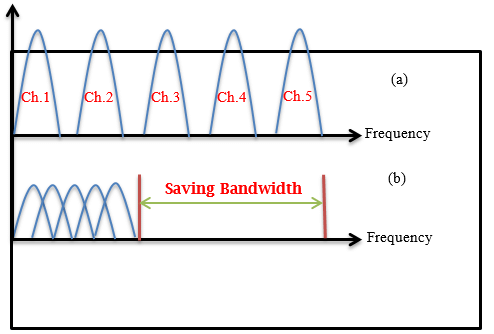
\includegraphics[width=0.92\textwidth]{Figures/multicarrier_concept.png}
    \caption{\bfseries Multicarrier technique versus Orthogonal Multicarrier technique}
    \label{fig:multicarrier}
\end{figure}

If the total system bandwidth is $B$ and the number of subcarriers is $N$,
then the bandwidth of each subcarrier becomes:

\begin{equation}
\Delta f = \frac{B}{N}
\end{equation}

As $N$ increases, each subcarrier experiences nearly flat fading, which
greatly simplifies equalization.

Orthogonal Frequency Division Multiplexing (OFDM) is the most widely used
multicarrier transmission scheme and forms the basis of many modern
wireless standards such as Wi-Fi, LTE, DVB, and 5G systems.

%============================================================%
\subsection{Wireless Multipath Fading Channels}

Wireless signals propagate through multiple paths due to reflection,
diffraction, and scattering from surrounding objects. The received signal
therefore becomes the superposition of several delayed and attenuated
copies of the transmitted waveform.

The channel impulse response of a multipath fading channel can be modeled
as:

\begin{equation}
h(t)=\sum_{l=0}^{L-1}\alpha_l \delta(t-\tau_l)
\end{equation}

where:
\begin{itemize}
    \item $L$ is the number of channel paths,
    \item $\alpha_l$ represents the complex gain of the $l$-th path,
    \item $\tau_l$ is the propagation delay,
    \item $\delta(\cdot)$ is the Dirac delta function.
\end{itemize}

The received signal is therefore expressed as:

\begin{equation}
r(t)=s(t)*h(t)+n(t)
\end{equation}

where:
\begin{itemize}
    \item $s(t)$ is the transmitted signal,
    \item $h(t)$ is the channel response,
    \item $n(t)$ denotes additive white Gaussian noise (AWGN).
\end{itemize}

\vspace{0.3cm}

\begin{figure}[H]
    \centering
    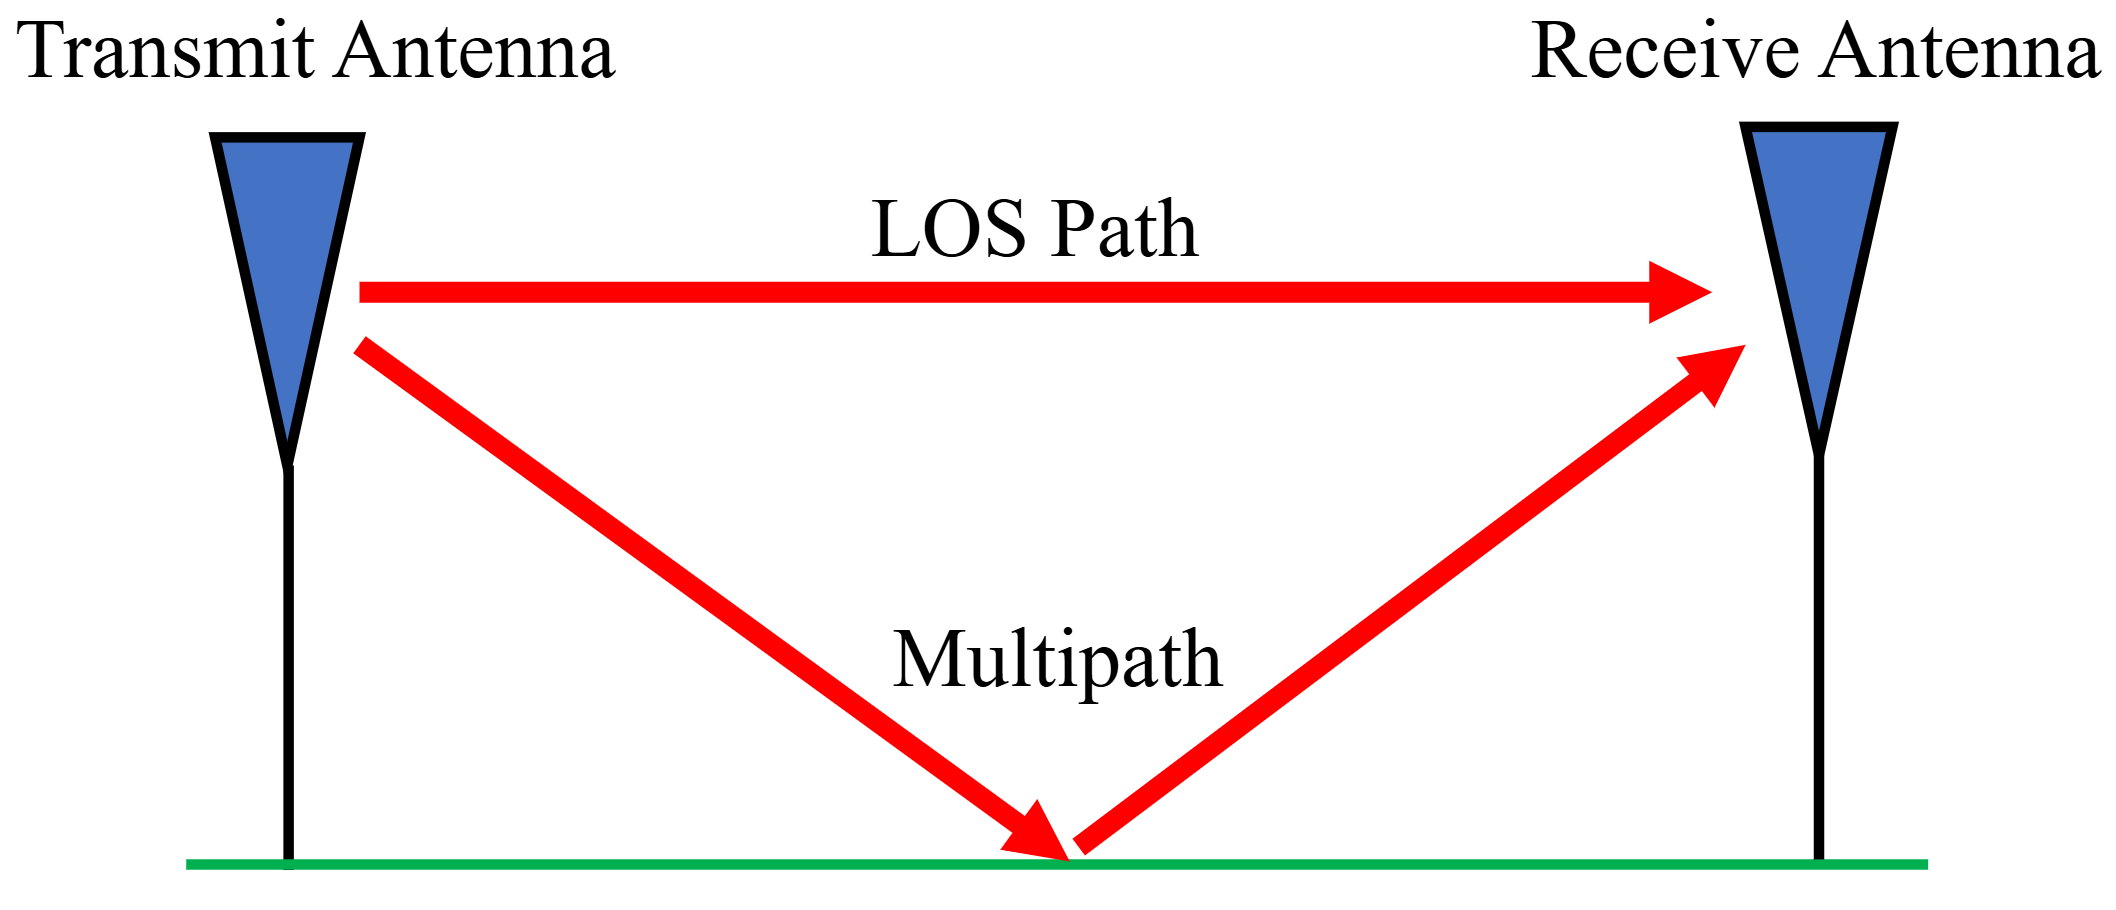
\includegraphics[width=0.92\textwidth]{Figures/rayleigh_channel.png}
    \caption{\bfseries Multipath fading channel model}
    \label{fig:rayleigh}
\end{figure}

When no dominant line-of-sight component exists, the channel envelope
typically follows a Rayleigh distribution. Such channels are commonly
called Rayleigh fading channels.

Frequency-selective fading occurs when different frequency components of
the signal experience different channel gains. OFDM and SC-FDMA were
developed specifically to combat this problem efficiently.

%============================================================%
%============================================================%
\subsection{Orthogonal Frequency Division Multiplexing (OFDM)}

Orthogonal Frequency Division Multiplexing (OFDM) is a multicarrier
transmission technique in which a high-rate data stream is divided into
multiple lower-rate parallel streams and transmitted simultaneously over
many orthogonal subcarriers.

Instead of using one high-bandwidth carrier, OFDM partitions the available
spectrum into narrowband subchannels. Because each subcarrier occupies a
small bandwidth, the effect of frequency-selective fading is significantly
reduced, and each subcarrier can be approximated as experiencing flat
fading.

OFDM has become one of the most important waveform technologies in modern
wireless communication systems and has been adopted in standards such as:

\begin{itemize}
    \item Wi-Fi (IEEE 802.11)
    \item LTE Downlink
    \item 5G NR
    \item DVB broadcasting systems
    \item ADSL and broadband wired communications
\end{itemize}

\vspace{0.3cm}

The basic OFDM transmitter structure is shown in
Figure~\ref{fig:ofdm_tx_rx}.

\vspace{0.3cm}

\begin{figure}[H]
    \centering
    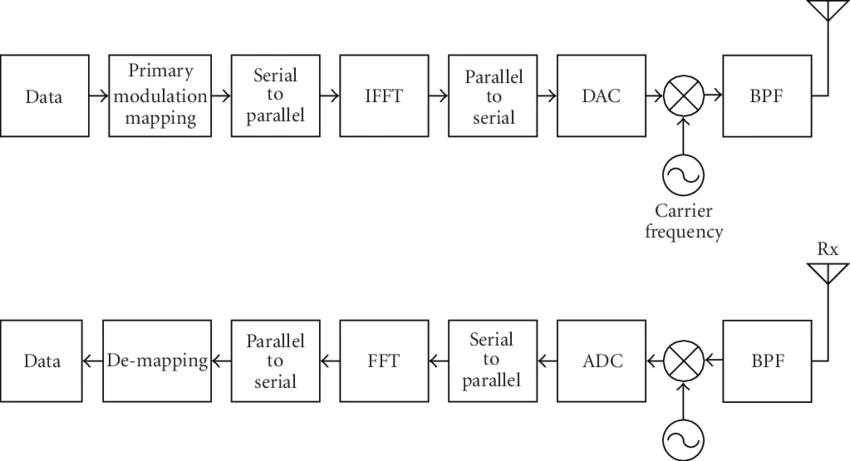
\includegraphics[width=0.95\textwidth]{Figures/ofdm_transmitter_receiver.png}
    \caption{\bfseries OFDM transmitter-receiver structure}
    \label{fig:ofdm_tx_rx}
\end{figure}

At the transmitter, the incoming serial bit stream is first converted into
parallel groups of bits and mapped into complex modulation symbols using
modulation schemes such as QPSK, 16-QAM, or 64-QAM.

Assume that:

\begin{equation}
X = [X[0],X[1],...,X[N-1]]
\end{equation}

represents the frequency-domain symbols assigned to the OFDM
subcarriers.

The OFDM modulator converts these symbols into a time-domain waveform
using the Inverse Fast Fourier Transform (IFFT):

\begin{equation}
x[n]=\frac{1}{N}\sum_{k=0}^{N-1}X[k]
e^{j\frac{2\pi kn}{N}}
\label{eq:ofdm_ifft}
\end{equation}

where:

\begin{itemize}
    \item $X[k]$ is the complex symbol transmitted on subcarrier $k$,
    \item $N$ is the total number of subcarriers,
    \item $x[n]$ is the discrete-time OFDM signal.
\end{itemize}

Equation~\ref{eq:ofdm_ifft} shows that the OFDM waveform is formed by the
superposition of many orthogonal sinusoidal carriers.

Because the subcarriers are orthogonal, they can overlap in the frequency
domain without causing inter-carrier interference (ICI). This allows OFDM
to achieve very high spectral efficiency compared to conventional
single-carrier systems.

\vspace{0.3cm}

At the receiver, the Fast Fourier Transform (FFT) operation converts the
received signal back into the frequency domain:

\begin{equation}
X[k]=\sum_{n=0}^{N-1}x[n]
e^{-j\frac{2\pi kn}{N}}
\label{eq:ofdm_fft}
\end{equation}

The FFT efficiently separates the orthogonal subcarriers and recovers the
transmitted data symbols.

\vspace{0.3cm}

The major advantages of OFDM include:

\begin{itemize}
    \item High spectral efficiency
    \item Excellent robustness against multipath fading
    \item Simple frequency-domain equalization
    \item Efficient implementation using FFT/IFFT algorithms
\end{itemize}

However, OFDM also suffers from several practical limitations:

\begin{itemize}
    \item High Peak-to-Average Power Ratio (PAPR)
    \item Sensitivity to carrier frequency offset
    \item Sensitivity to synchronization errors
\end{itemize}

Among these limitations, high PAPR is considered one of the most critical
issues in practical transmitter implementation.

%============================================================%
\subsection{Orthogonality of Subcarriers}

The key principle behind OFDM is orthogonality between subcarriers.

Although the subcarriers overlap in the frequency domain, they remain
mathematically independent over one symbol duration. This property enables
multiple subcarriers to share the same bandwidth efficiently without
mutual interference.

Two continuous-time subcarriers are orthogonal if:

\begin{equation}
\int_0^T
e^{j2\pi(f_k-f_m)t}dt = 0
\qquad k \neq m
\label{eq:orthogonality}
\end{equation}

where:

\begin{itemize}
    \item $f_k$ and $f_m$ are different subcarrier frequencies,
    \item $T$ is the OFDM symbol duration.
\end{itemize}

To satisfy this condition, adjacent subcarriers are separated by:

\begin{equation}
\Delta f = \frac{1}{T}
\label{eq:subcarrier_spacing}
\end{equation}

This spacing guarantees that the peak of one subcarrier coincides with the
zero crossings of neighboring subcarriers.

\vspace{0.3cm}

\begin{figure}[H]
    \centering
    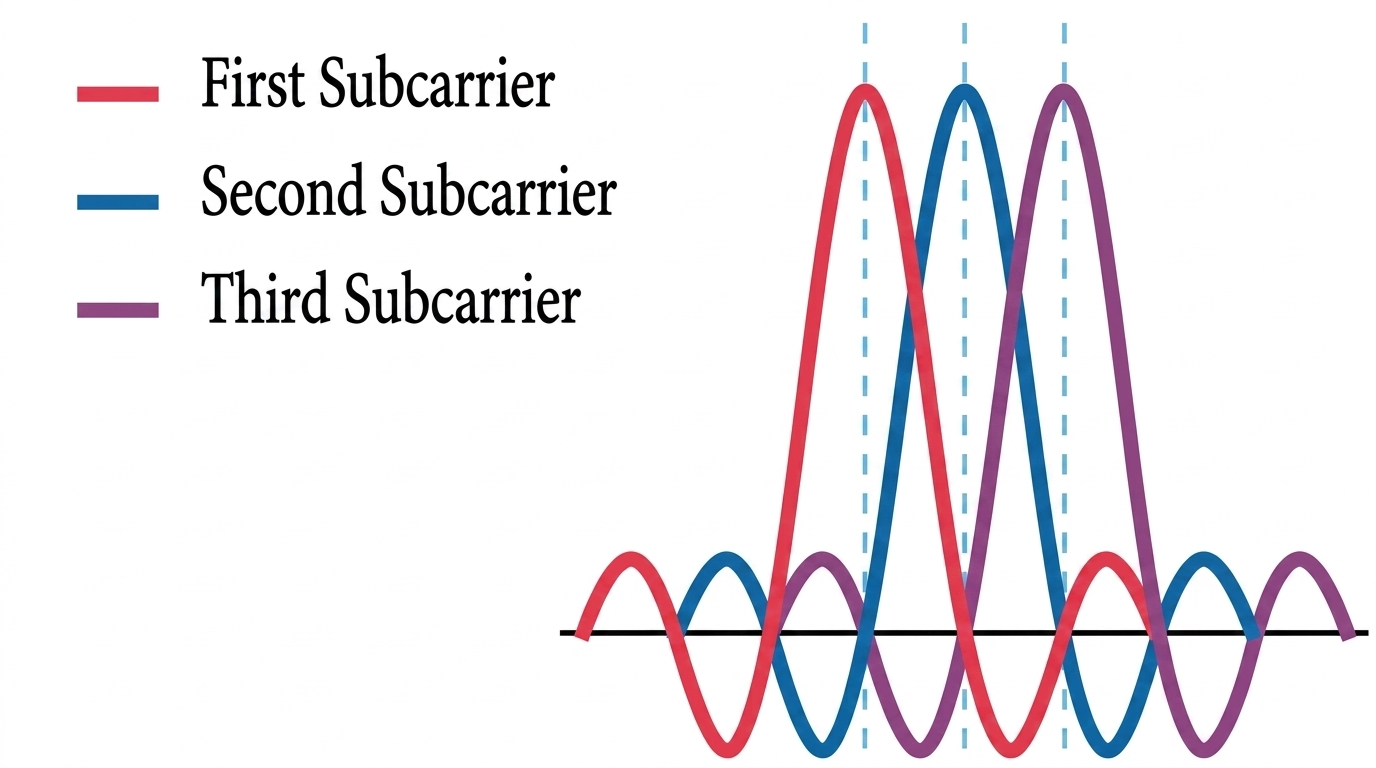
\includegraphics[width=0.62\textwidth]{Figures/orthogonal_subcarriers.png}
    \caption{\bfseries Orthogonality between adjacent OFDM subcarriers}
    \label{fig:orthogonality}
\end{figure}

Figure~\ref{fig:orthogonality} illustrates how orthogonal subcarriers
overlap spectrally while remaining separable at the receiver.

This property significantly improves spectrum utilization compared to
traditional Frequency Division Multiplexing (FDM), where large guard bands
are required between channels.

%============================================================%
\subsection{Cyclic Prefix (CP)}

Wireless channels often contain multiple delayed signal paths caused by
reflection, diffraction, and scattering.

As a result, delayed replicas of previous OFDM symbols may overlap with
the current symbol and create Inter-Symbol Interference (ISI).

To combat ISI, OFDM inserts a Cyclic Prefix (CP) before each OFDM symbol.

The CP is created by copying the final portion of the OFDM symbol and
appending it to the beginning of the transmitted block.

If the CP length exceeds the maximum channel delay spread, the linear
convolution between the channel and transmitted signal becomes circular
convolution:

\begin{equation}
y[n]=x[n]\circledast h[n]
\label{eq:circular_conv}
\end{equation}

where:

\begin{itemize}
    \item $x[n]$ is the transmitted OFDM symbol,
    \item $h[n]$ is the channel impulse response,
    \item $y[n]$ is the received signal.
\end{itemize}

This transformation is extremely important because circular convolution in
the time domain corresponds to simple multiplication in the frequency
domain:

\begin{equation}
Y[k]=X[k]H[k]
\label{eq:freq_domain_channel}
\end{equation}

As a result, equalization becomes very simple since each subcarrier only
requires a one-tap equalizer:

\begin{equation}
\hat{X}[k]=\frac{Y[k]}{H[k]}
\label{eq:equalization}
\end{equation}

\vspace{0.3cm}

\begin{figure}[H]
    \centering
    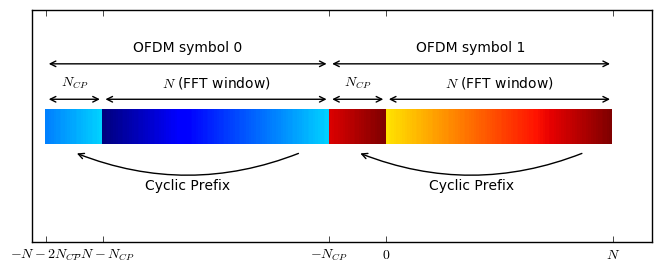
\includegraphics[width=0.9\textwidth]{Figures/cyclic_prefix.png}
    \caption{\bfseries Cyclic prefix insertion in OFDM systems}
    \label{fig:cp}
\end{figure}

The figure above illustrates two consecutive OFDM symbols, where each
symbol contains its own cyclic prefix. The CP is a replica of the final
samples of the OFDM block.

At the receiver, the FFT window begins after the cyclic prefix is removed.
If the CP duration is sufficiently long, delayed channel components remain
inside the guard interval and do not corrupt the useful OFDM symbol.

Although the cyclic prefix improves robustness against multipath fading,
it also introduces overhead and slightly reduces spectral efficiency.

%============================================================%
\subsection{Single-Carrier Frequency Division Multiple Access (SC-FDMA)}

Single-Carrier Frequency Division Multiple Access (SC-FDMA) is a modified
version of OFDM designed to reduce Peak-to-Average Power Ratio (PAPR).

SC-FDMA is also commonly referred to as:

\begin{itemize}
    \item DFT-spread OFDM (DFT-s-OFDM)
    \item Single-Carrier OFDM (SC-OFDM)
\end{itemize}

Unlike conventional OFDM, SC-FDMA inserts a Discrete Fourier Transform
(DFT) operation before subcarrier mapping.

This additional processing spreads each modulation symbol across multiple
subcarriers before OFDM modulation.

Because of this spreading effect, the transmitted waveform exhibits
single-carrier characteristics with reduced envelope fluctuation.

The transmitter and receiver structures are illustrated in
Figure~\ref{fig:scfdma_tx_rx}.

\vspace{0.3cm}

\begin{figure}[H]
    \centering
    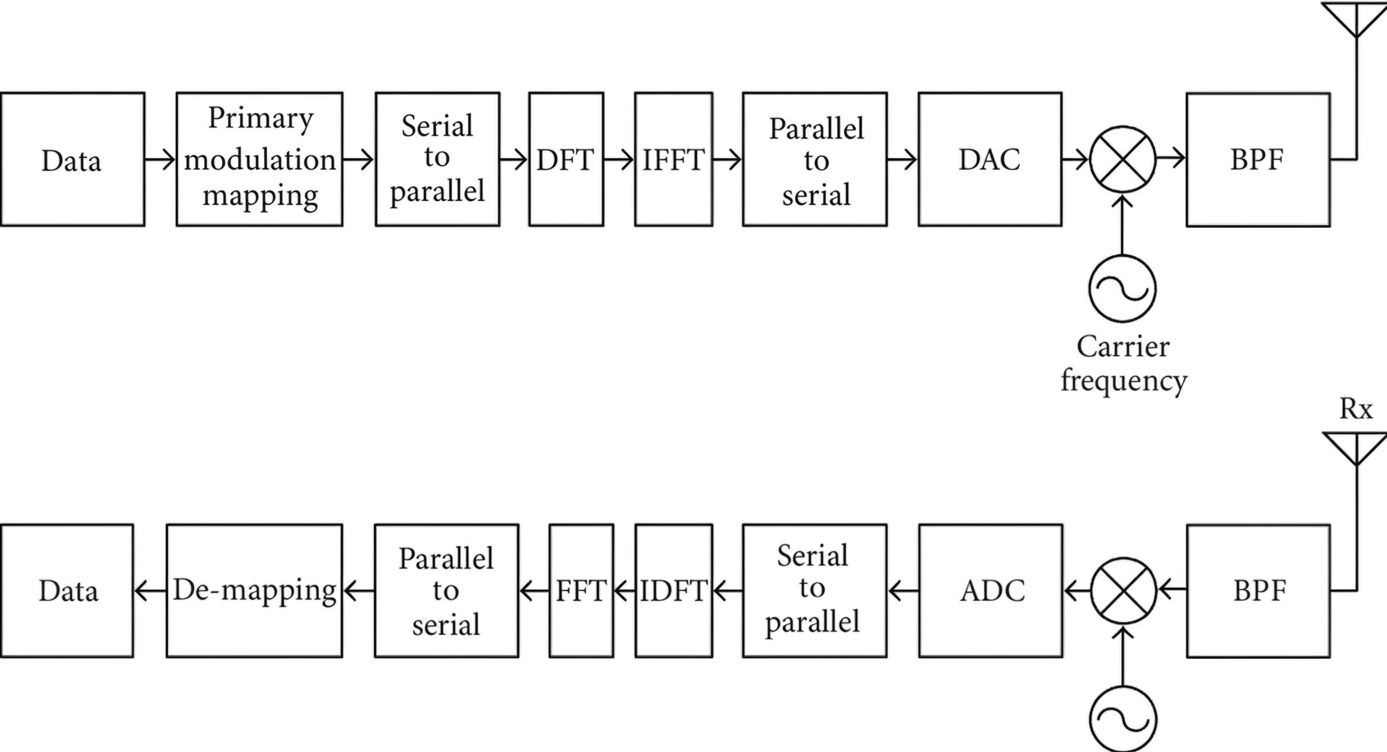
\includegraphics[width=0.95\textwidth]{Figures/scfdma_transmitter_receiver.png}
    \caption{\bfseries SC-FDMA transmitter-receiver structure}
    \label{fig:scfdma_tx_rx}
\end{figure}

At the transmitter, the modulated symbols are first transformed using an
$M$-point DFT:

\begin{equation}
X[m]=\sum_{n=0}^{M-1}
d[n]e^{-j\frac{2\pi mn}{M}}
\label{eq:dft_spreading}
\end{equation}

where:

\begin{itemize}
    \item $d[n]$ is the input modulation symbol,
    \item $X[m]$ is the DFT-spread symbol,
    \item $M$ is the number of occupied subcarriers.
\end{itemize}

The spread symbols are then mapped onto OFDM subcarriers before the IFFT
operation.

The resulting time-domain signal becomes:

\begin{equation}
x[n]=
\frac{1}{N}
\sum_{k=0}^{N-1}
X[k]
e^{j\frac{2\pi kn}{N}}
\label{eq:scfdma_signal}
\end{equation}

Although Equation~\ref{eq:scfdma_signal} appears mathematically similar
to OFDM, the important difference is that the input symbols have already
been precoded by the DFT operation.

This DFT spreading distributes information symbols across the occupied
subcarriers and significantly reduces instantaneous signal peaks.

\vspace{0.3cm}

At the receiver, the cyclic prefix is removed and FFT processing is
performed similarly to OFDM.

After subcarrier demapping, an inverse DFT (IDFT) operation reconstructs
the original modulation symbols:

\begin{equation}
d[n]=\frac{1}{M}
\sum_{m=0}^{M-1}
X[m]e^{j\frac{2\pi mn}{M}}
\label{eq:idft_despreading}
\end{equation}

The complete receiver chain can therefore be summarized as:

\begin{center}
Remove CP $\rightarrow$ FFT $\rightarrow$
Subcarrier Demapping $\rightarrow$
IDFT $\rightarrow$ Symbol Detection
\end{center}

One major advantage of SC-FDMA is lower PAPR compared to OFDM.

In OFDM, multiple independently phased subcarriers may occasionally add
constructively, creating very large peaks in the transmitted waveform.

In SC-FDMA, DFT spreading introduces correlation between subcarriers,
making the transmitted waveform resemble a single-carrier signal with
smaller amplitude variation.

This property improves power amplifier efficiency and reduces nonlinear
distortion.

For this reason, SC-FDMA was selected as the uplink waveform in LTE mobile
communication systems, where battery efficiency is critically important.

\vspace{0.3cm}

SC-FDMA also exhibits improved robustness against localized spectral nulls
caused by frequency-selective fading.

In OFDM, severe fading on one subcarrier directly destroys the information
carried on that subcarrier.

In SC-FDMA, information symbols are spread across multiple subcarriers.
Therefore, fading on a single subcarrier affects all symbols only
partially rather than completely destroying one symbol.

However, SC-FDMA also introduces several tradeoffs:

\begin{itemize}
    \item Additional DFT/IDFT processing complexity
    \item More complicated subcarrier mapping structures
    \item Slightly less flexibility compared to OFDM
\end{itemize}

Despite these tradeoffs, the lower PAPR characteristic makes SC-FDMA
highly suitable for uplink mobile transmission systems.

%============================================================%
\subsection{Localized SC-FDMA Mapping}

There are two main SC-FDMA subcarrier mapping methods:

\begin{itemize}
    \item Localized FDMA (LFDMA)
    \item Interleaved FDMA (IFDMA)
\end{itemize}

In localized mapping, consecutive subcarriers are allocated to a user:

\begin{equation}
k = 0,1,2,\dots,M-1
\end{equation}

In interleaved mapping, subcarriers are distributed uniformly across the
entire bandwidth:

\begin{equation}
k = 0,L,2L,\dots,(M-1)L
\end{equation}

where $L$ is the subcarrier spacing interval.

This report focuses only on localized SC-FDMA because it is more commonly
used in LTE uplink systems.

\vspace{0.3cm}

\begin{figure}[H]
    \centering
    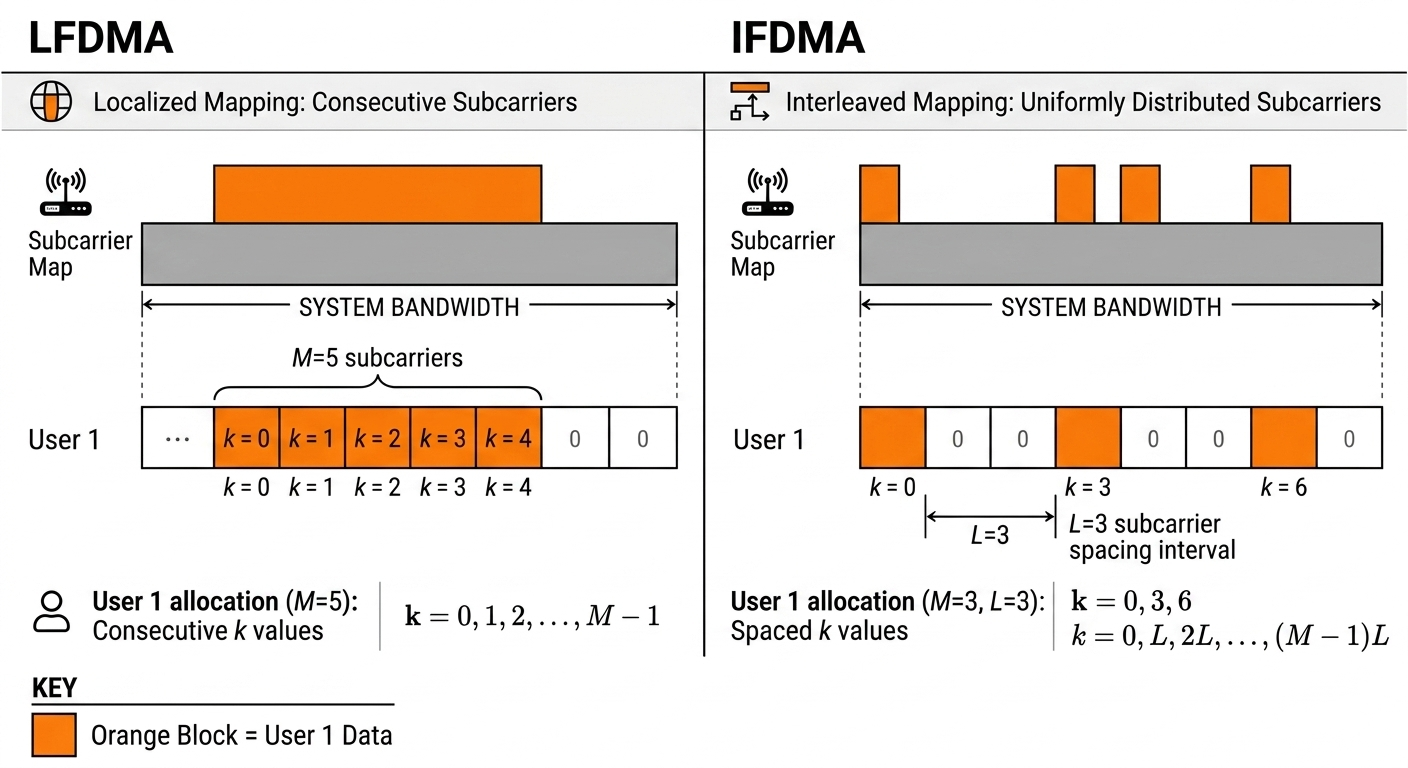
\includegraphics[width=0.95\textwidth]{Figures/scfdma_mapping.png}
    \caption{\bfseries Localized versus interleaved SC-FDMA subcarrier allocation}
    \label{fig:mapping}
\end{figure}

%============================================================%
\subsection{Peak-to-Average Power Ratio (PAPR)}

PAPR measures the ratio between the maximum instantaneous signal power and
its average power.

Mathematically:

\begin{equation}
\mathrm{PAPR}
=
\frac{\max |x[n]|^2}
{E\{|x[n]|^2\}}
\end{equation}

PAPR is usually expressed in decibels:

\begin{equation}
\mathrm{PAPR}_{dB}
=
10\log_{10}
\left(
\frac{\max |x[n]|^2}
{E\{|x[n]|^2\}}
\right)
\end{equation}

In OFDM systems, independently phased subcarriers occasionally combine
constructively, creating large signal peaks.

According to the central limit theorem, the OFDM signal amplitude tends
toward a Gaussian distribution as the number of subcarriers increases.

SC-FDMA reduces this effect because DFT spreading introduces correlation
between transmitted samples, producing a waveform closer to conventional
single-carrier transmission.

%============================================================%
\subsection{Complementary Cumulative Distribution Function (CCDF)}

The Complementary Cumulative Distribution Function (CCDF) is commonly used
to evaluate PAPR statistics.

CCDF represents the probability that the signal PAPR exceeds a threshold
value $P_0$:

\begin{equation}
\mathrm{CCDF}(P_0)
=
\Pr(\mathrm{PAPR}>P_0)
\end{equation}

A lower CCDF curve indicates lower probability of high signal peaks and
better power amplifier efficiency.

%============================================================%
\subsection{Frequency-Domain Equalization}

Multipath fading distorts the transmitted signal differently across
subcarriers. Equalization is therefore necessary to compensate for channel
effects.

After FFT demodulation, the received signal on the $k$-th subcarrier is:

\begin{equation}
Y[k]=H[k]X[k]+N[k]
\end{equation}

where:
\begin{itemize}
    \item $H[k]$ is the channel frequency response,
    \item $X[k]$ is the transmitted symbol,
    \item $N[k]$ is additive noise.
\end{itemize}

In Zero Forcing (ZF) equalization, the estimated transmitted symbol is:

\begin{equation}
\hat{X}[k]=\frac{Y[k]}{H[k]}
\end{equation}

ZF equalization completely removes channel distortion under ideal channel
estimation conditions. However, it may significantly amplify noise when
$H[k]$ becomes very small.

\vspace{0.3cm}

%\begin{figure}[H]
%    \centering
%    \includegraphics[width=0.92\textwidth]{Figures/zf_equalizer.png}
%    \caption{\bfseries Frequency-domain Zero Forcing equalization}
%    \label{fig:zf}
%\end{figure}

%============================================================%
\subsection{Bit Error Rate (BER)}

Bit Error Rate (BER) measures communication reliability by comparing the
number of incorrectly detected bits to the total transmitted bits.

\begin{equation}
\mathrm{BER}
=
\frac{N_e}{N_t}
\end{equation}

where:
\begin{itemize}
    \item $N_e$ is the number of erroneous bits,
    \item $N_t$ is the total number of transmitted bits.
\end{itemize}

Lower BER indicates better system performance.

In this report, BER under different Signal-to-Noise Ratio (SNR)
conditions is used to compare OFDM and SC-FDMA performance in multipath
fading channels.

%============================================================%
\subsection{Comparison Summary}

\begin{table}[H]
\centering
\caption{Comparison between OFDM and SC-FDMA}
\begin{tabularx}{\textwidth}
{|>{\raggedright\arraybackslash}X|
 >{\centering\arraybackslash}X|
 >{\centering\arraybackslash}X|}
\hline
\textbf{Criterion} & \textbf{OFDM} & \textbf{SC-FDMA} \\ \hline

Transmission Structure
& Pure multicarrier
& DFT-spread multicarrier \\ \hline

PAPR
& High
& Lower \\ \hline

Power Amplifier Efficiency
& Lower
& Higher \\ \hline

Equalization Complexity
& Simple
& Simple \\ \hline

Frequency Diversity
& Limited to subcarrier
& Spread across subcarriers \\ \hline

Implementation Complexity
& Lower
& Slightly Higher \\ \hline

LTE Usage
& Downlink
& Uplink \\ \hline

\end{tabularx}
\end{table}

%============================================================%
\subsection{Chapter Summary}

This chapter presented the theoretical foundations of OFDM and SC-FDMA,
including multicarrier transmission principles, multipath fading channels,
orthogonality, cyclic prefix operation, DFT spreading, PAPR analysis,
CCDF evaluation, and frequency-domain equalization.

The next chapter presents the MATLAB simulation model and analyzes the BER
and PAPR performance of OFDM and SC-FDMA systems under multipath Rayleigh
fading channels.